% !TeX encoding = UTF-8

% 载入 SJTUThesis 模版
\documentclass[type=master]{sjtuthesis}
% 选项
%   type=[doctor|master|bachelor],     % 可选(默认:master),论文类型
%   zihao=[-4|5],                      % 可选(默认:-4),正文字号大小
%   lang=[zh|en|de|ja],                % 可选(默认:zh),论文的主要语言
%   review,                            % 可选(默认:关闭),盲审模式
%   [twoside|oneside],                 % 可选(默认:twoside),双页或单页边距模式
%   [openright|openany],               % 可选(默认:openright),奇数页或任意页开始新章
%   math-style=[ISO|TeX],              % 可选 (默认:ISO),数学符号样式

% 论文基本配置,加载宏包等全局配置
% !TEX root = ./main.tex

\sjtusetup{
  %
  %******************************
  % 注意:
  %   1. 配置里面不要出现空行
  %   2. 不需要的配置信息可以删除
  %******************************
  %
  % 信息录入
  %
  info = {%
    %
    % 标题
    %
    zh / title           = {基于先验信息的实时三维介入CT重建},
    en / title           = {Real-time 3D Interventional CT Reconstruction Based on Prior Information},
    %
    % 标题页标题
    %   可使用“\\”命令手动控制换行
    %
    % zh / display-title   = {上海交通大学学位论文\\ \LaTeX{} 模板示例文档},
    % en / display-title   = {A Sample Document \\ for \LaTeX-based SJTU Thesis Template},
    %
    % 关键词
    %
    zh / keywords        = {CT重建, 深度学习, 先验信息},
    en / keywords        = {CT Reconstruction, Deep Learning, Prior Information},
    %
    % 姓名
    %
    zh / author          = {裴奕博},
    en / author          = {Yibo Pei},
    %
    % 指导教师
    %
    zh / supervisor      = {赵俊,全国涛},
    en / supervisor      = {Prof.\ Jun Zhao and Prof.\ Guotao Quan},  
    %
    % 副指导教师
    %
    % zh / assoc-supervisor  = {某某教授},
    % en / assoc-supervisor  = {Prof.\ Uom Uom},
    %
    % 学号
    %
    id              = {122082910048},
    %
    % 学位
    %   除交叉学科门类外,各一级学科按所属学科门类申请学位
    %   专业学位类别按专业名称申请学位
    %   本科生不需要填写
    %
    zh / degree          = {工学硕士},
    en / degree          = {Master of Engineering},
    %
    % 专业
    %
    zh / major           = {电子信息类},
    en / major           = {Electronics and Information Engineering},
    %
    % 所属院系
    %
    zh / department      = {生物医学工程学院},
    en / department      = {School of Biomedical Engineering},
    %
    % 答辩日期
    %   使用 ISO 格式 (yyyy-mm-dd);默认为当前时间
    %
    % date                 = {2023-05-18},
    %
    % 标题页显示日期
    %   覆盖对应标题页的日期显示,原样输出
    %
    % zh / display-date    = {2023 年 5 月},
    %
    % 资助基金
    zh / fund  = {
                 {国家自然科学基金 (No.\ 92059206)},
                 },
    en / fund  = {
                   {National Natural Science Foundation of China (Grant No.\ 92059206)},
                 },
  },
  %
  % 风格设置
  %
  style = {%
    %
    % 关键词首行悬挂
    %
    % keywords-format = hang,
  },
  %
  % 名称设置
  %
  name = {
    % bib             = {References},
    % ack             = {谢\hspace{\ccwd}辞},
    % achv            = {攻读学位期间完成的论文},
  },
}

% 使用 BibLaTeX 处理参考文献
%   biblatex-gb7714-2015 常用选项
%     gbnamefmt=lowercase     姓名大小写由输入信息确定
%     gbpub=false             禁用出版信息缺失处理
\usepackage[backend=biber,style=gb7714-2015]{biblatex}
% 文献表字体
\renewcommand{\bibfont}{\zihao{5}\setbaselineskip{16bp}}
% 文献表条目间的间距
\setlength{\bibitemsep}{3bp plus 1pt}
% 导入参考文献数据库
\addbibresource{refs.bib}

% 脚注格式
\usepackage[perpage,bottom,hang]{footmisc}

% 定义图片文件目录与扩展名
\graphicspath{{figures/}}
\DeclareGraphicsExtensions{.pdf,.eps,.png,.jpg,.jpeg}

% 确定浮动对象的位置,可以使用 [H],强制将浮动对象放到这里(可能效果很差)
% \usepackage{float}

% 固定宽度的表格
% \usepackage{tabularx}

% 使用三线表:toprule,midrule,bottomrule。
\usepackage{booktabs}

% 表格中支持跨行
\usepackage{multirow}

% 表格中数字按小数点对齐
\usepackage{dcolumn}
\newcolumntype{d}[1]{D{.}{.}{#1}}

% 使用长表格
\usepackage{longtable}

% 附带脚注的表格
\usepackage{threeparttable}

% 附带脚注的长表格
\usepackage{threeparttablex}

% 算法环境宏包
\usepackage[ruled,vlined,linesnumbered]{algorithm2e}
% \usepackage{algorithm, algorithmicx, algpseudocode}

% 代码环境宏包
\usepackage{listings}
\lstdefinestyle{lstStyleCode}{%
  aboveskip         = \medskipamount,
  belowskip         = \medskipamount,
  basicstyle        = \ttfamily\zihao{-5}\setbaselineskip{12bp},
  commentstyle      = \slshape\color{black!60},
  stringstyle       = \color{green!40!black!100},
  keywordstyle      = \bfseries\color{blue!50!black},
  extendedchars     = false,
  upquote           = true,
  tabsize           = 2,
  showstringspaces  = false,
  xleftmargin       = 1em,
  xrightmargin      = 1em,
  breaklines        = false,
  framexleftmargin  = 1em,
  framexrightmargin = 1em,
  backgroundcolor   = \color{gray!10},
  columns           = flexible,
  keepspaces        = true,
  texcl             = true,
  mathescape        = true
}
\lstnewenvironment{codeblock}[1][]{%
  \lstset{style=lstStyleCode,#1}}{}

% 直立体数学符号
\providecommand{\dd}{\mathop{}\!\mathrm{d}}
\providecommand{\ee}{\mathrm{e}}
\providecommand{\ii}{\mathrm{i}}
\providecommand{\jj}{\mathrm{j}}

% 国际单位制宏包
\usepackage{siunitx}

% 定理环境宏包
\usepackage{amsthm}
% \usepackage{ntheorem}

% 绘图宏包
\usepackage{tikz}
\usetikzlibrary{arrows.meta, shapes.geometric}

% 数据图表宏包
\usepackage{pgfplots}
\pgfplotsset{compat=newest}

% 一些文档中用到的 logo
\usepackage{hologo}
\providecommand{\XeTeX}{\hologo{XeTeX}}
\providecommand{\BibLaTeX}{\textsc{Bib}\LaTeX}

% 借用 ltxdoc 里面的几个命令方便写文档
\DeclareRobustCommand\cs[1]{\texttt{\char`\\#1}}
\providecommand\pkg[1]{{\sffamily#1}}

% hyperref 宏包在最后调用
\usepackage{hyperref}

% E-mail
\providecommand{\email}[1]{\href{mailto:#1}{\urlstyle{tt}\nolinkurl{#1}}}


\begin{document}

%TC:ignore

% 标题页
\maketitle

% 原创性声明及使用授权书
\copyrightpage
% 插入外置原创性声明及使用授权书
% 此时必须在导言区使用 \usepackage{pdfpages}
% \copyrightpage[scans/sample-copyright.pdf]

% 前置部分
\frontmatter

% 摘要
\input{contents/abstract}

% 目录
\tableofcontents*
% 插图索引
\listoffigures*
% 表格索引
\listoftables*
% 算法索引
\listofalgorithms*

% 符号对照表
% !TEX root = ../main.tex

\begin{nomenclature*}
\label{chap:symb}

\begin{longtable}{rl}
  $\epsilon$  & 介电常数  \\
  $\mu$       & 磁导率    \\
\end{longtable}

\end{nomenclature*}


%TC:endignore

% 主体部分
\mainmatter

% 正文内容
% !TEX root = ../main.tex

\chapter{绪论}

\section{研究背景及意义}
\subsection{介入手术中的CT引导}
介入放射学(Interventional Radiology, IR),是一门在医学影像的实时引导下,利用穿刺针、导管、支架等介入器材,对疾病进行诊断或治疗的学科\cite{TengGaoJunJieRuZhiLiaoXue2022}。自从1940年代世界上第一例经皮肾脏穿刺术成功进行以来,经过半个多世纪的发展,介入放射学已经发展为对于放射学乃至医学界最重要的先进技术之一,其近年来的发展和进步也非常活跃\cite{HuXiaoKunZhangFuJunXiaoYueYongCTJieRuZhiLiaoXue2020}。由于介入诊断和治疗具有定位精确、创口小、减少病患痛苦等优势,随着介入放射学与临床关系愈发密切,介入放射学已经能够为患者提供更加微创和安全有效的医学诊断和治疗方法,在特定领域已经代替了传统的诊断和治疗方式。

根据介入目的的不同,介入放射学可分为两大分支:介入诊断学和介入治疗学。在介入放射学发展的早期,医生主要将其用于获取人体生物组织样本,即通过穿刺活检或抽取体液来进行病理学分析以诊断疾病。比较具有代表性的介入诊断方式有血管造影、胆管造影和活检等。随着技术发展,介入放射学也开始深入治疗领域。根据治疗器官和部位的不同,包括血管介入(血管支架/球囊植入、血管内动脉瘤修复、溶栓等)、肝胆介入、消化道介入以及泌尿生殖系统介入等。根据介入诊疗中所需的影像设备不同,又可以分为数字减影血管造影(Digital Subtraction Angoigraphy,DSA)介入、CT介入、超声介入及磁共振介入等。

计算机断层成像(Computed Tomography,CT),是一种利用人体不同组织对X射线的吸收不同实现的断层成像技术,被广泛应用于各类诊断和治疗领域。CT断层图像解决了传统数字化摄影(Digital Radiology,DR)的前后混叠问题,可提供病灶和器官的高分辨率精细结构。此外,相比超声介入的低分辨率和磁共振介入费用昂贵且需要专用介入器械,CT引导的介入(CT Guided Intervention)在介入诊断和治疗中具有突出的优势。在介入手术的过程中,CT引导技术可分为两种:常规CT引导和实时CT透视引导(Real-time CT Fluoroscopy,RTCT)。常规CT引导技术实现了3D影像的快速重建和显示,使得穿刺活检和治疗的安全性得到了提高,然而由于其非实时性,常规CT影像容易受到呼吸、心跳等人体生理运动的干扰而发生偏移,因此单次进针穿刺的成功率不高。此外,术中医生需要往返于扫描机间和CT控制室,操作流程较为繁琐。为了解决非实时性的问题,1994年Katada等人发明了RTCT,相比传统CT,RTCT具有更快的扫描和重建速度,可以在进针时提供实时的影像引导,大大提升了单次进针的成功率,是未来临床应用的方向\cite{HuXiaoKunZhangFuJunXiaoYueYongCTJieRuZhiLiaoXue2020,katadaDevelopmentRealtimeCT1994}。

\subsection{介入CT重建算法及存在的问题}
相比传统的诊断用CT,介入CT重建在保持重建原理不变的同时,对于实时性提出了更高的要求,目前临床上RTCT引导可达到每秒约6-15帧。根据重建算法的原理,常见的CT重建算法可分为以滤波反投影(Filtered Back Projection,FBP)重建、代数重建(Algebra Reconstruction Technique,ART)或称基于模型的迭代重建(Model-based Iterative Reconstruction,MBIR)、以及近年来兴起的基于深度学习的CT重建(Deep Learning Reconstruction,DLR)。其中,基于模型的迭代重建由于其重建速度的限制,无法胜任介入手术。近年来,随着人工智能和计算机视觉的飞速发展,基于深度学习的CT重建算法由于其具有图像质量好、推理速度快的优势,在介入CT重建领域也有着广泛的应用前景。基于深度学习的重建算法在诊断用CT上已经进入临床实用阶段,但对于RTCT的针对性优化和实际使用仍然不太成熟,因此目前在临床应用中,重建算法仍然以传统的FBP算法为主。传统的FBP算法具有原理简单,重建速度快等优势,在CT重建领域长期作为基准方法使用。但由于RTCT的特殊性,其在剂量、分辨率和伪影等方面仍然存在诸多问题。

首先是X射线的剂量问题。一次正常剂量CT的扫描剂量可以达到43mSv,是人体本底辐射的100倍以上\cite{smith-bindmanRadiationDoseAssociated2009}。然而在介入手术过程中,患者和医生在几分钟内均需要暴露在X射线下,持续时间显著长于诊断用CT,因此患者受到的辐射剂量也会大幅提升。为了避免高额的辐射剂量给患者和医生带来的潜在危险,RTCT通常会使用低剂量扫描的方式,但这会不可避免的损失图像质量。然而,即便是这样,研究发现,使用低剂量扫描的一次RTCT胸部穿刺剂量平均为79mGy,仍然远远超过一次胸部CT平扫的30mGy剂量\cite{HuXiaoKunZhangFuJunXiaoYueYongCTJieRuZhiLiaoXue2020}。受限于手术需求和医生的介入操作时长,X射线的照射时长很难缩短,因此如何进一步降低RTCT引导的辐射剂量,成为了一个有价值的问题。

其次是介入手术过程中产生的伪影问题。与人体组织相比,金属具有更高的密度和原子序数。受到射束硬化、光子饥饿、散射辐射、部分容积效应以及金属本身运动等多重因素影响,会在整个CT影像中产生全局性的伪影\cite{demanMetalStreakArtifacts1999}。由于金属的形态和运动方式的不同,金属伪影可呈现条状、星状等多样的形态\cite{hsiehComputedTomographyPrinciples2022}。这些伪影相比真实影像CT值可相差数百HU,会极大影响临床医生的视野和判断。在介入CT中,通常医生都需要使用金属制成的穿刺针深入到特定的组织位置,且相比患者体内的金属植入物(如心脏起搏器、内固定钢板等)运动状态更加复杂,因此会时刻伴随较大的金属伪影问题。

\begin{figure}[!htp]
  \centering
  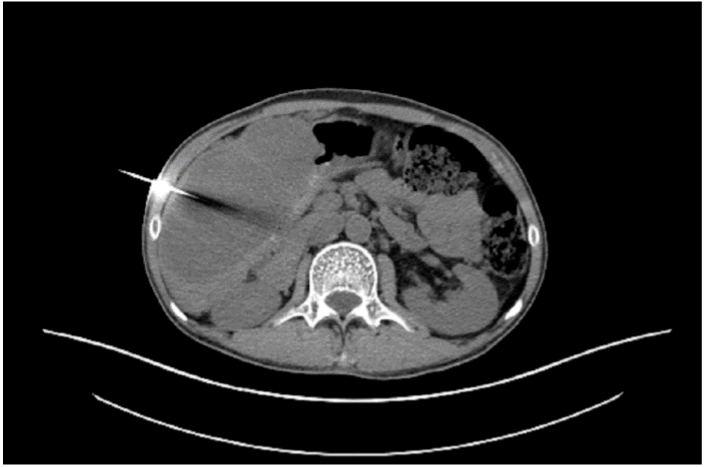
\includegraphics[width=0.6\textwidth]{RTCT.png}
  \bicaption{介入手术的CT引导影像(图中可见金属伪影)}{CT-guided image in Interventional Radiology (metal artifact visible)}
  \label{fig. RTCT}
\end{figure}

此外还有时间分辨率和空间分辨率的矛盾问题。CT成像的最大优势是其较高的空间分辨率,目前主流诊断用CT的x-y方向空间分辨率及层厚均已可达到0.5mm,然而这样的高分辨率只能在完整扫描数据和薄层CT重建的情况下才能得以实现。一方面,由于RTCT引导过程中通常采用低剂量扫描,空间分辨率显然不如完整数据的诊断CT。此外,在临床上最常用的FBP算法在低剂量CT的重建问题上表现显著不如代数重建和深度学习算法,其重建结果通常会伴随较大的噪声。另一方面,由于对于实时性的高要求,在实际的RTCT引导中,为了加快FBP算法的重建速度,通常只能采用减少层厚并降低x-y方向分辨率的方式实现实时的穿刺引导,空间分辨率仅可维持在5mm左右。因此目前基于FBP的介入CT重建算法,实际上限制了硬件上可获得的时空分辨率。因此,如何在保证实时性的同时,为介入医生提供更高的组织分辨率,是介入CT重建算法需要解决的重要问题。

综上所述,由于RTCT的实时引导三维断层成像定位准确、显示清晰,CT引导的介入在介入放射学中占有重要地位。然而在临床实际应用中,最常用的FBP重建算法在介入CT的特定环境下仍然存在辐射剂量、时空分辨率、金属伪影等多方面亟待解决的问题。因此,本课题旨在研究一种高分辨率和低伪影的介入CT重建算法,为临床医生提供介入操作时高分辨率的实时引导,并最大程度的降低医生和病患所受的辐射剂量。具体来说,本文的研究存在以下几个方面的挑战:
\begin{enumerate}
  \item 当前的介入手术已经普遍采用LDCT扫描,但由于持续时间较长医生和患者仍然会暴露在长时间的辐射下。如何在保证图像质量的情况下,最大程度的降低患者和医生所受的辐射剂量。
  \item 介入手术中的金属器械会造成金属伪影干扰医生判断。如何更好的去除介入过程中产生的金属伪影,从而避免对医生产生干扰。
  \item 介入手术和低剂量扫描给重建算法提出了更高的要求。如何在高空间分辨率与重建的实时性要求上达到平衡,以便更好地为医生提供介入手术的引导。
\end{enumerate}

\section{国内外研究现状}
随着深度学习和计算机视觉的发展,基于人工智能的医学影像处理得到了迅速发展。这些问题包括低剂量CT重建、去金属伪影等CT重建和后处理问题,均已经有了许多深入的研究。生成对抗网络\cite{goodfellowGenerativeAdversarialNets2014}和Transformer\cite{vaswaniAttentionAllYou2017}等近年来火热的计算机视觉网络结构,也已经在医学图像处理中得到了广泛应用。下面我将对这些已有的研究现状进行综述。

\subsection{低剂量CT重建算法}
根据奈奎斯特采样定律,降低采样率会降低图像的信噪比,影响后续重建得到的图像质量。传统的FBP算法在LDCT重建上难以获得令人满意的结果,重建图像会出现明显的条状伪影。目前主流的LDCT重建算法可以分为正弦图滤波、图像域后处理、基于模型的迭代(Model-based Iterative Reconstruction,MBIR)以及基于深度学习的LDCT重建。

正弦图滤波试图在正弦图去除伪影,再使用传统算法重建到图像域。其中常用的方法有自适应滤波、双边滤波等。Balda等人提出了一种结构自适应正弦图(Structure Adaptive Sinogram,SAS)滤波器,使用基于点的前向投影来生成一种称为射线贡献掩模(Radiation Contribution Mask, RCM)的局部结构表示。在不改变重建算法和不引入伪影的情况下,SAS滤波器将噪声水平降低了13.6\% \cite{baldaRayContributionMasks2012}。然而,投影域中任何模型偏差或不恰当的操作都会引入全局干扰,影响正弦图滤波结果的准确性和鲁棒性。

图像域后处理直接对重建完成后的CT影像进行操作,通常需要利用一些图像的先验假设。Chen等人提出了一种基于图像块的快速字典学习算法,改善了腹部肿瘤的LDCT影像,并以低于常规CT扫描1/5的剂量保留了肿瘤特征\cite{chenImprovingAbdomenTumor2013}。Chen等人还提出了通过大规模邻域加权强度平均法(Weighted Intensity Averaging over Large-scale Neighborhoods,WIA-LN)来改进LDCT图像的方法,使用大规模邻域内属于不同器官或衰减组织的像素的选择性加权强度平均值作为去除噪声之后的像素值\cite{chenImprovingLowdoseXray2010}。然而,这类通常更适用于自然图像处理的方法在医学影像上具有天然劣势:重建后的图像伪影会由于反投影操作而在整张图片中不均匀分布,且这种噪声不遵循已知分布,无法直接解析建模。因此,图像域后处理方法的效果事实上比较有限。

MBIR算法结合了以上两种方法的优点,其核心是一个待优化的目标函数,通常情况下包含两项:投影域的带噪声的保真项和图像域的带有先验的正则项。比较主流的方法包括全变分(Total Variation,TV)\cite{rudinNonlinearTotalVariation1992}、惩罚加权最小二乘 (Penalized Weighted-least Squares,PWLS )\cite{sauerLocalUpdateStrategy1993} 和压缩感知(Conpressive Sensing,CS)\cite{donohoCompressedSensing2006}算法等。Yu等人将TV准则引入CT重建领域,并使用水平集算法求得数值解\cite{yuTotalVariationBased2005}。Chen等人提出了先验图像约束的压缩感知算法(Prior Image Constrained Compressed Sensing,PICCS),利用动态CT成像中的时空相关性对动态CT图像序列进行稀疏化,并将压缩感知方法应用于目标图像序列的重建\cite{chenPriorImageConstrained2008}。Xu等人利用字典学习,将冗余字典的稀疏约束纳入到目标函数中。该字典既可以在图像重建任务之前预先确定,也可以在重建过程中自适应定义\cite{xuLowDoseXrayCT2012}。Zheng等人将PWLS和基于稀疏变换(Sparsifying Transform,ST)的正则化相结合,交替优化PWLS-ST代价函数,显著提高了重建图像的质量\cite{zhengLowDoseCT2016}。MBIR算法在传统方法中取得了较好的效果,获得图像的噪声相比FBP有了显著提升,然而迭代算法的计算成本高昂,重建时间约在数分钟左右,这一点对于实时成像的RTCT来说几乎是不可接受的,因此目前在临床上仍未在已有的介入CT扫描中直接使用。

近年来,深度学习算法也逐渐开始被应用于医学影像领域,目前对于低剂量CT重建也已经有了大量的研究。深度学习算法由于其端到端的便利性,极高的图像质量以及较快的重建速度体现出了强大的优势。比较常用的重建框架结构包括卷积神经网络(Convolutional Neural Network,CNN)、U-Net\cite{ronnebergerUNetConvolutionalNetworks2015}以及生成对抗网络(Generative Adversarial Network,GAN)\cite{goodfellowGenerativeAdversarialNets2014}等。根据图像处理方式的不同,如图~\ref{fig. DLR}所示,目前基于深度学习的LDCT重建可以大体分为四种不同的类别:图像域处理、投影域处理、双域重建以及直接重建。

\begin{figure}[!htp]
  \centering
  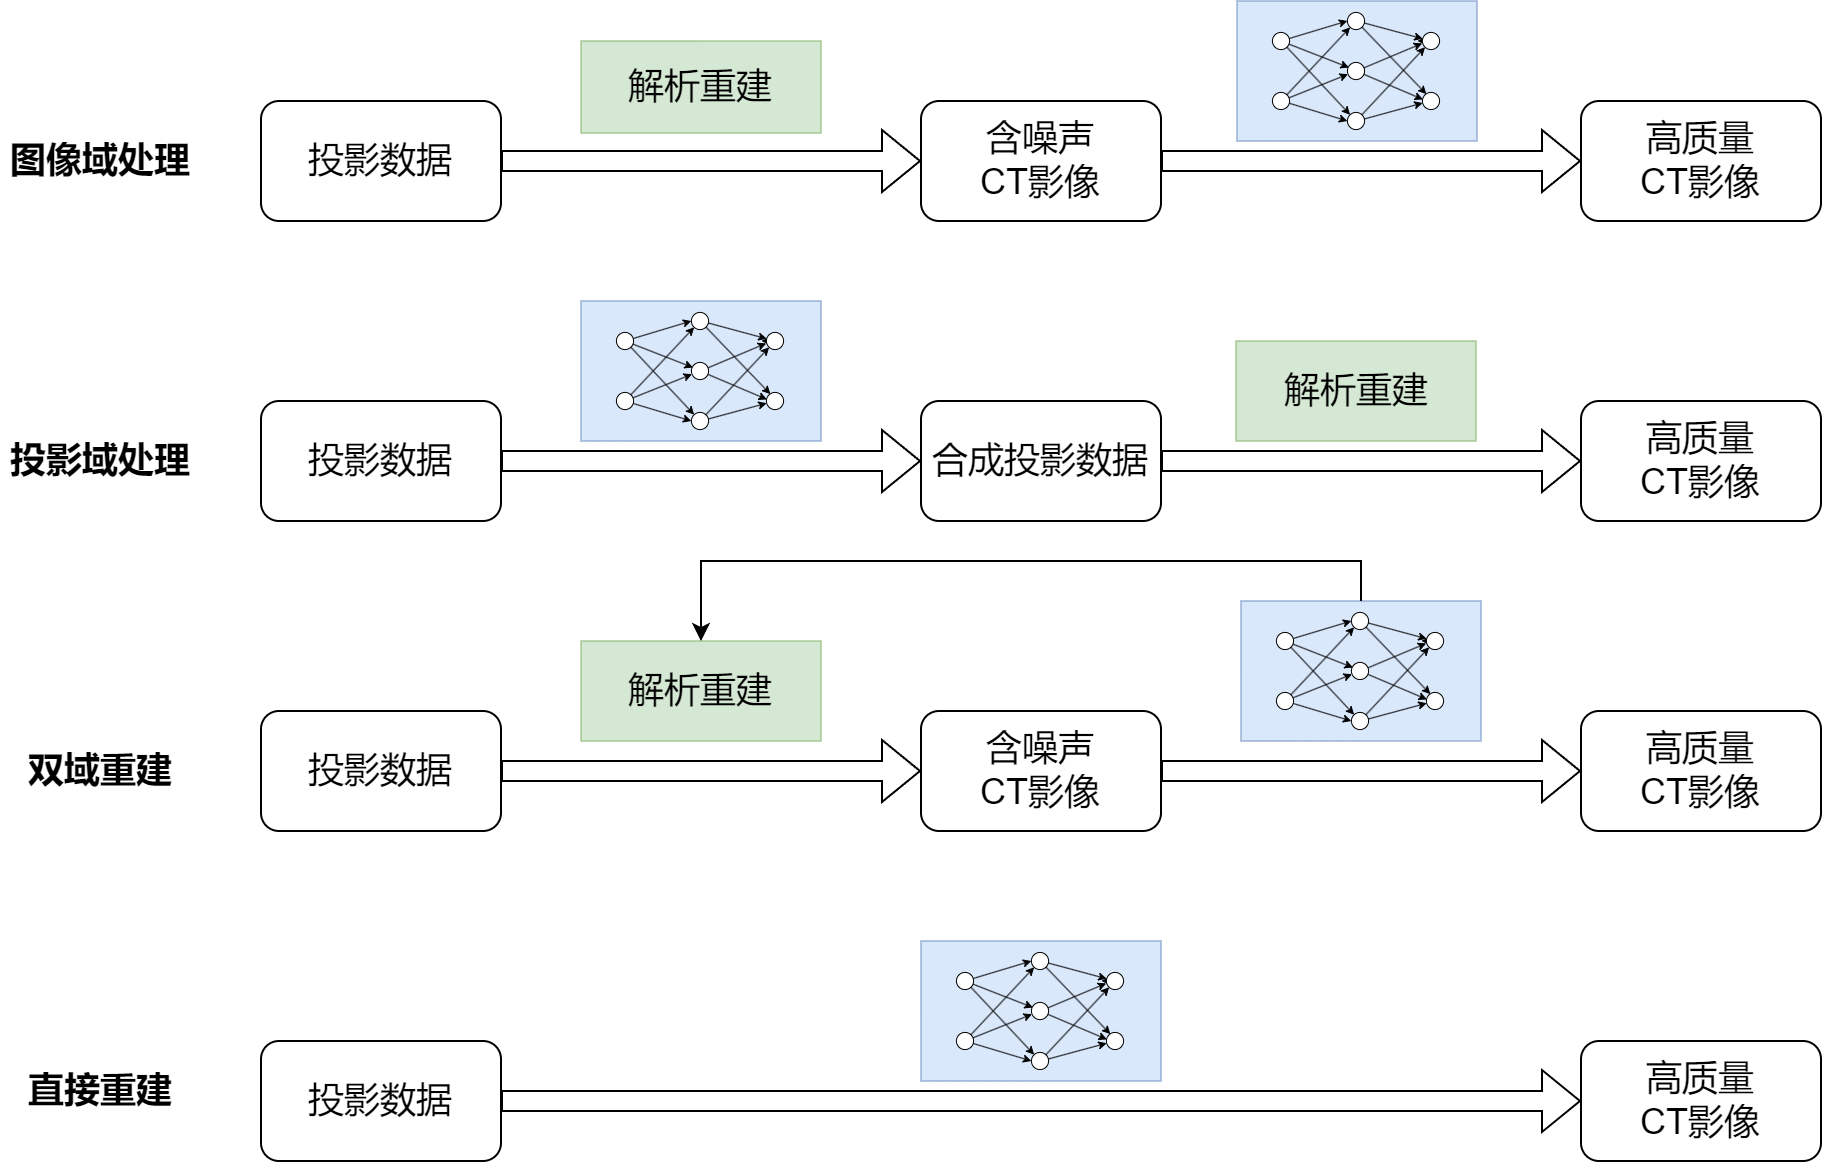
\includegraphics[width=\textwidth]{DLR.drawio.png}
  \bicaption{基于深度学习的低剂量CT重建分类}{The Classification of Deep Learning LDCT Reconstruction Methods}
  \label{fig. DLR}
\end{figure}

在深度学习重建方法中,被报道最多的方法是图像域的处理方法。这种方法使用深度神经网络对欠采样的重建图像进行去噪。Cheng等人结合了自编码器、反卷积和跳跃连接,提出了残差自编码器卷积神经网络(Residual Encoder-decoder Convolutional Neural Network ,RED-CNN),在噪声抑制、结构保持和病灶检测方面都得到了较好的效果\cite{chenLowDoseCTResidual2017}。Xie等人使用改进的GoogLeNet\cite{szegedyGoingDeeperConvolutions2015},去除稀疏角度CT重建中由于投影缺失而产生的条形伪影,恢复出清晰的重建图像\cite{xieArtifactRemovalUsing2018}。Wolterink等人使用生成对抗网络,有效提升了含钙模体和非增强扫描心脏CT的图像质量,允许在高噪声水平的LDCT图像中进行冠状动脉钙化评分\cite{wolterinkGenerativeAdversarialNetworks2017}。Jin等人提出了基于U-Net的FBPConvNet,并在低至50个视图的稀疏视图CT重建问题上验证了性能\cite{jinDeepConvolutionalNeural2017}。Kang等人利用小波变换提取伪影的方向分量,并结合深度学习网络U-Net,有效地从LDCT图像中去除复杂的噪声\cite{kangDeepConvolutionalNeural2017}。Zhang等人提出了TransCT,分离含噪声图像的高频和低频图像并分别提取特征后输入Transformer\cite{vaswaniAttentionAllYou2017},得到了优越的效果\cite{zhangTransCTDualPathTransformer2021}。图像域重建的优点是思路直接,可以移植大量在计算机视觉领域已经证明有效的成熟模型。然而其缺点也很明显:在重建时需要首先依赖FBP或者迭代算法得到含噪声的图像,这一过程可能导致信息的丢失,限制了最终重建的结果。

投影域方法的目标是将原本稀疏角度的投影图修复成完整的投影图,然后再使用FBP等解析方式进行重建。Liang等人利用残差学习,搭建了一个多分支的投影角度恢复网络,得到了条状伪影显著降低的重建图像\cite{liangImproveAngularResolution2018}。Liu等人使用Pix2Pix GAN\cite{isolaImageToImageTranslationConditional2017}对投影图进行修复,得到的结果显著优于直接插值得到的结果\cite{liuSparsesamplingCTSinogram2020}。然而,基于投影域的方法仍然无法摆脱传统方法的限制,想得到更加纯净的重建图像需要做进一步后处理。

双域方法结合了以上二者的优点。Feng等人提出MDD-U-net,使用U-Net修复LDCT的正弦图,并结合了投影域和图像域两部分损失,在保留图像细节的同时更有效的去除了噪声\cite{fengPreliminaryStudyProjection2020a}。Yuan等人提出的SIPID网络交替进行投影域的修复和图像域的后处理,取得了比纯图像域去噪更好的效果\cite{yuanSIPIDDeepLearning2018}。Cheng等人提出FSR-Net,通过对CT图像和投影数据进行正则化,并引入一种新的全采样条件来融合来自双域的信息,结合迭代算法实现了端到端的图像重建\cite{chengLearnedFullSamplingReconstruction2020a}。双域方法有效整合了投影域和图像域两方面的信息,理论上能取得更好的效果,然而过于复杂的结构给训练和数据集提出了更高的要求。

最后是直接使用深度神经网络学习投影正弦图到图像域重建图像映射的直接深度学习方法。Zhu等人提出的AUTOMAP模型使用神经网络学习从测量域到图像域的转换方式,并在磁共振成像(Magnetic Resonance Imaging,MRI)数据集上得到了验证\cite{zhuImageReconstructionDomaintransform2018}。基于这个设想,Kandarpa等人提出了DUG-RECON模型,该模型由去噪、重建和超分辨率三个级联的网络组成。在其中的重建网络部分,使用一个双U-Net生成器学习正弦图到重建影像的转换,在LDCT和正电子发射计算机断层扫描(Positron Emission Computed Tomography,PET)影像数据集成功进行了可行性验证\cite{kandarpaDUGRECONFrameworkDirect2021}。此类方法无需借助传统的FBP或者迭代算法,结构简单。然而这也同时意味着舍弃了重建过程中的物理信息,神经网络需要学习更加复杂的映射模式,给网络结构的设计带来了更大的困难。另外,当投影角度极其稀疏时(如小于10个时的极端情况),由于输入信息中物理信息的缺失,因此需要使用这样的直接深度学习方法。


\subsection{基于GAN和Transformer的医学影像重建}
近年来,随着计算机视觉的飞速发展,以卷积神经网络(Convolutional Neural Network,CNN)为代表的深度学习技术在医学图像领域中得到了越来越广泛的应用。相比传统的图像处理和机器学习算法,深度学习无需人工构建特征,可以直接从原始数据中学习到更高层次的特征表示,实现端到端的图像处理和生成,实现更精确的结果预测。生成对抗网络(Generative Adversarial Network,GAN)和Transformer是近年来计算机视觉领域的两大热门网络结构,分别在自然图像生成和自然语言处理领域取得了巨大成功,今年来也已经在医学图像处理中得到了广泛的应用。

GAN是由Goodfellow等人\cite{goodfellowGenerativeAdversarialNets2014}于2014年提出的一种生成模型,其核心结构如图\ref{fig. GAN}所示,其核心思想是通过两个网络的对抗训练,一个生成器网络负责生成数据,一个判别器网络负责判断生成的数据是否为真实数据。在训练过程中,生成器网络通过生成尽可能逼真的数据来欺骗判别器网络,而判别器网络则通过判断生成的数据是否为真实数据来提高自己的判断能力。经过多轮的对抗训练,生成器网络可以生成逼真的数据。在医学图像重建领域,GAN也已经得到了广泛的应用。

\begin{figure}[!htp]
  \centering
  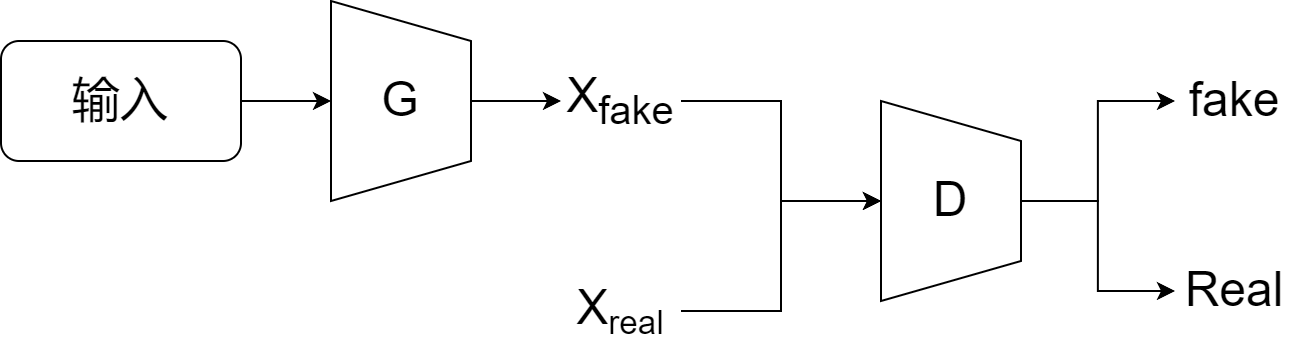
\includegraphics[width=0.6\textwidth]{GAN.drawio.png}
  \bicaption{生成对抗网络结构示意}{GAN Structure}
  \label{fig. GAN}
\end{figure}

% TODO: GAN在医学影像处理中的应用

Transformer\cite{vaswaniAttentionAllYou2017}是一种由自注意力机制驱动的新型深度学习模块,最初被应用于机器翻译、文本摘要等自然语言处理(NLP)任务。该模型的创新之处在于引入了注意力机制(Attention Mechanism),其设计思路摒弃了传统循环神经网络(Recurrent Neural Networks, RNN)和长短时记忆网络(Long-short Time Memory, LSTM)的顺序依赖性,使得信息处理能够实现并行化,从而在效率与性能上取得突破。Transformer的核心组成部份包括多头自注意力(Multi-Head Self-Attention)模块和前馈全连接层(Feed-forward Neural Networks)。多头自注意力机制允许模型通过多个并行的注意力子模块来分别关注输入序列的不同方面,这一设计使得模型能够捕捉更加复杂且多元的信息关联,提高了表征学习的能力。而前馈全连接层则作为非线性变换器,负责在经过多头注意力处理后提取出的关键信息上进行深度特征映射。此外,Transformer还创新性地引入了位置编码(Positional Encoding)机制,以编码序列元素间的相对顺序关系,确保模型能够理解文本的结构。为了优化训练过程并防止过拟合,残差连接(Residual Connections)和层归一化(Layer Normalization)等技术也被整合入模型架构中。Transformer不仅实现了在多项NLP任务上的性能飞跃,也揭示了深度学习处理序列数据的新路径。


\begin{figure}[!htp]
  \centering
  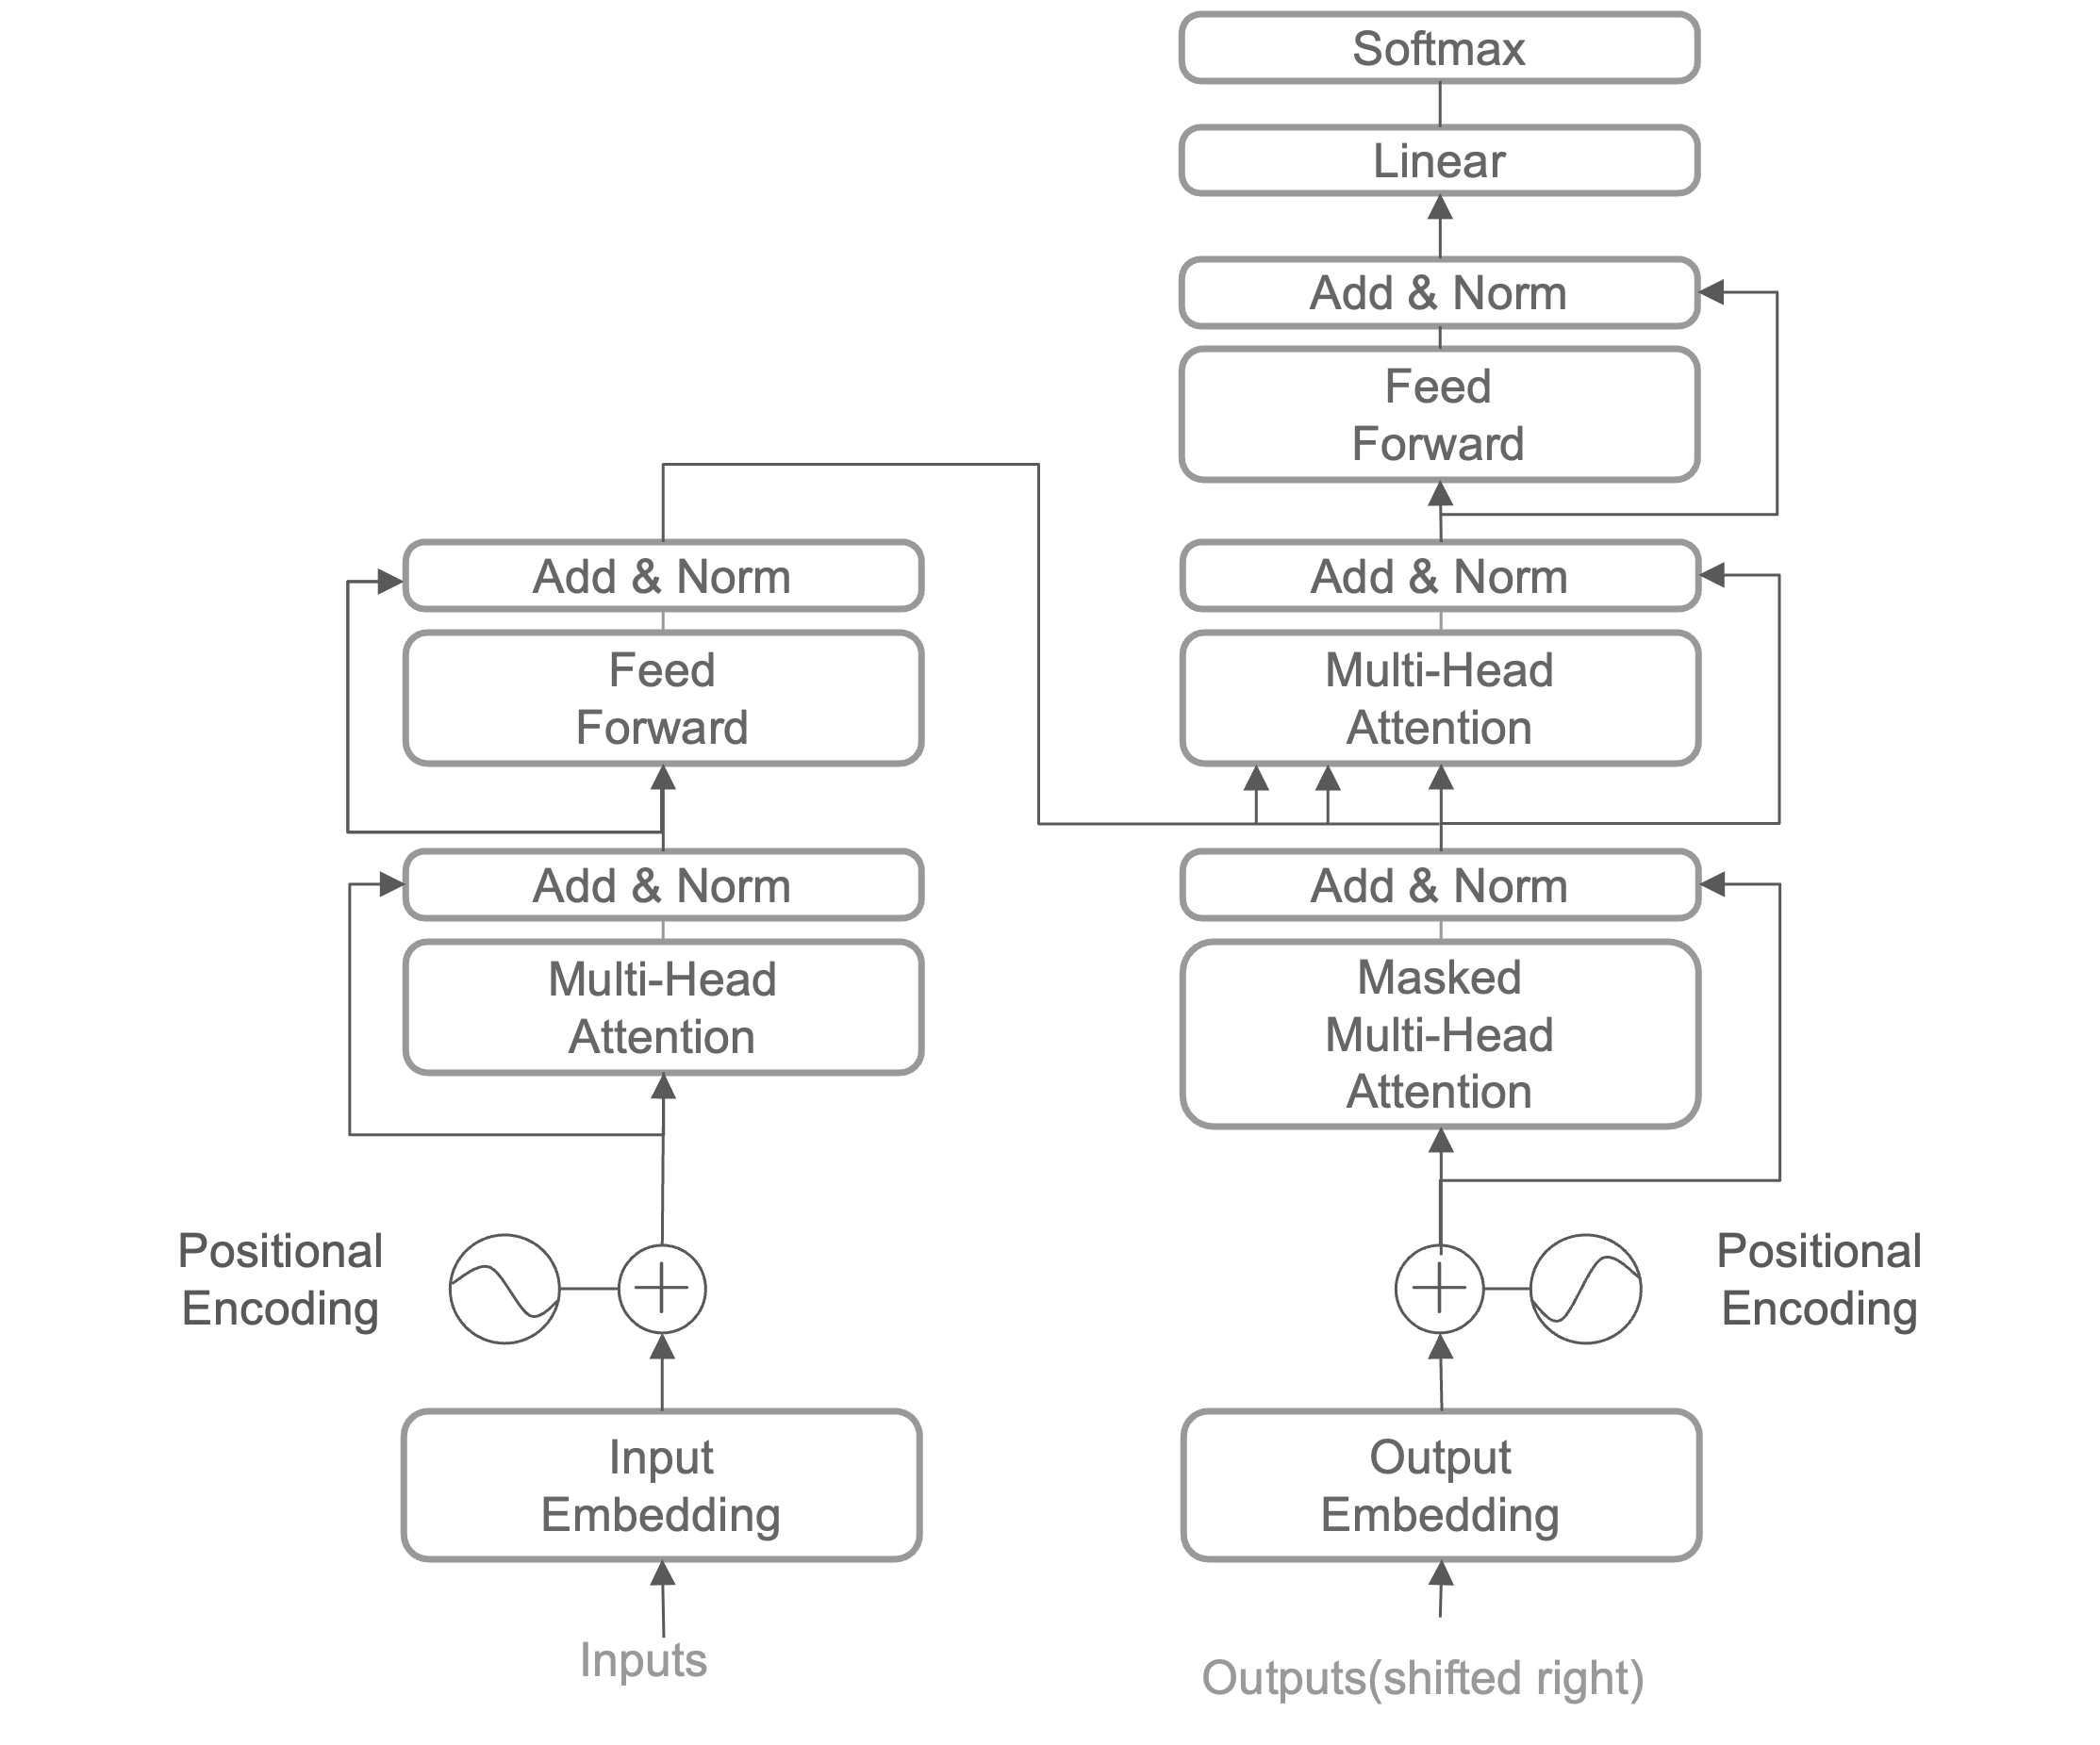
\includegraphics[width=0.6\textwidth]{Transformer.png}
  \bicaption{Transformer网络结构示意}{Transformer Structure}
  \label{fig. Transformer}
\end{figure}


2021年,Dosovitskiy等人提出了Vision Transformer(ViT)\cite{dosovitskiyImageWorth16x162021a},将图像切分成若干个可编码的小块,将Transformer这一强大技术引入到计算机视觉任务重中。近年来,ViT已经被应用于医学图像处理的各个方面,包括图像重建\cite{shenCOTRConvolutionTransformer2021,zhangTransCTDualPathTransformer2021,wangDuDoTransDualDomainTransformer2022,caoSwinUnetUnetLikePure2023,heH2FormerEfficientHierarchical2023,huangMISSFormerEffectiveTransformer2023,wangMISSU3DMedical2023,dalmazResViTResidualVision2022,wangTRCTGANCTReconstruction2023}。相较于CNN,Transformer的优势在于其对长距离特征的表示和捕捉能力,这使其在许多医学成像任务中具有竞争优势。例如,TransCT\cite{zhangTransCTDualPathTransformer2021}利用Transformer架构从噪声LDCT图像中提取高频和低频特征,然后将其用于分段重建方法,实现LDCT图像的去噪和增强。DuDoTrans\cite{wangDuDoTransDualDomainTransformer2022}集成了Transformer和CNN架构,利用它们各自捕捉长距离和短距离特征的能力从稀疏视图中恢复正弦图,从而成功在图像域重建CT图像。TRCT-GAN\cite{wangTRCTGANCTReconstruction2023}将Transformer应用于超稀疏CT重建领域。在这个框架中,Transformer 用于增强 X 射线图像中的特征表示,而动态注意模块用于加强上下文相关性,从而有效地从双平面X射线图像重建CT切片数据。

\subsection{直线检测方法研究现状}
% TODO: 直线检测方法研究现状
\section{主要研究内容和贡献}
本文针对术中介入CT扫描重建的问题,提出了一种两步骤的介入CT重建算法。如图\ref{fig. content}所示,首先使用术中超稀疏定位片并结合术前先验重建术中扫描的三维解剖结果,再使用直线检测方法进行术中介入针定位最终得到高分辨率和无伪影的介入术中CT重建影像。主要研究内容和贡献如下:

\begin{figure}[!htp]
  \centering
  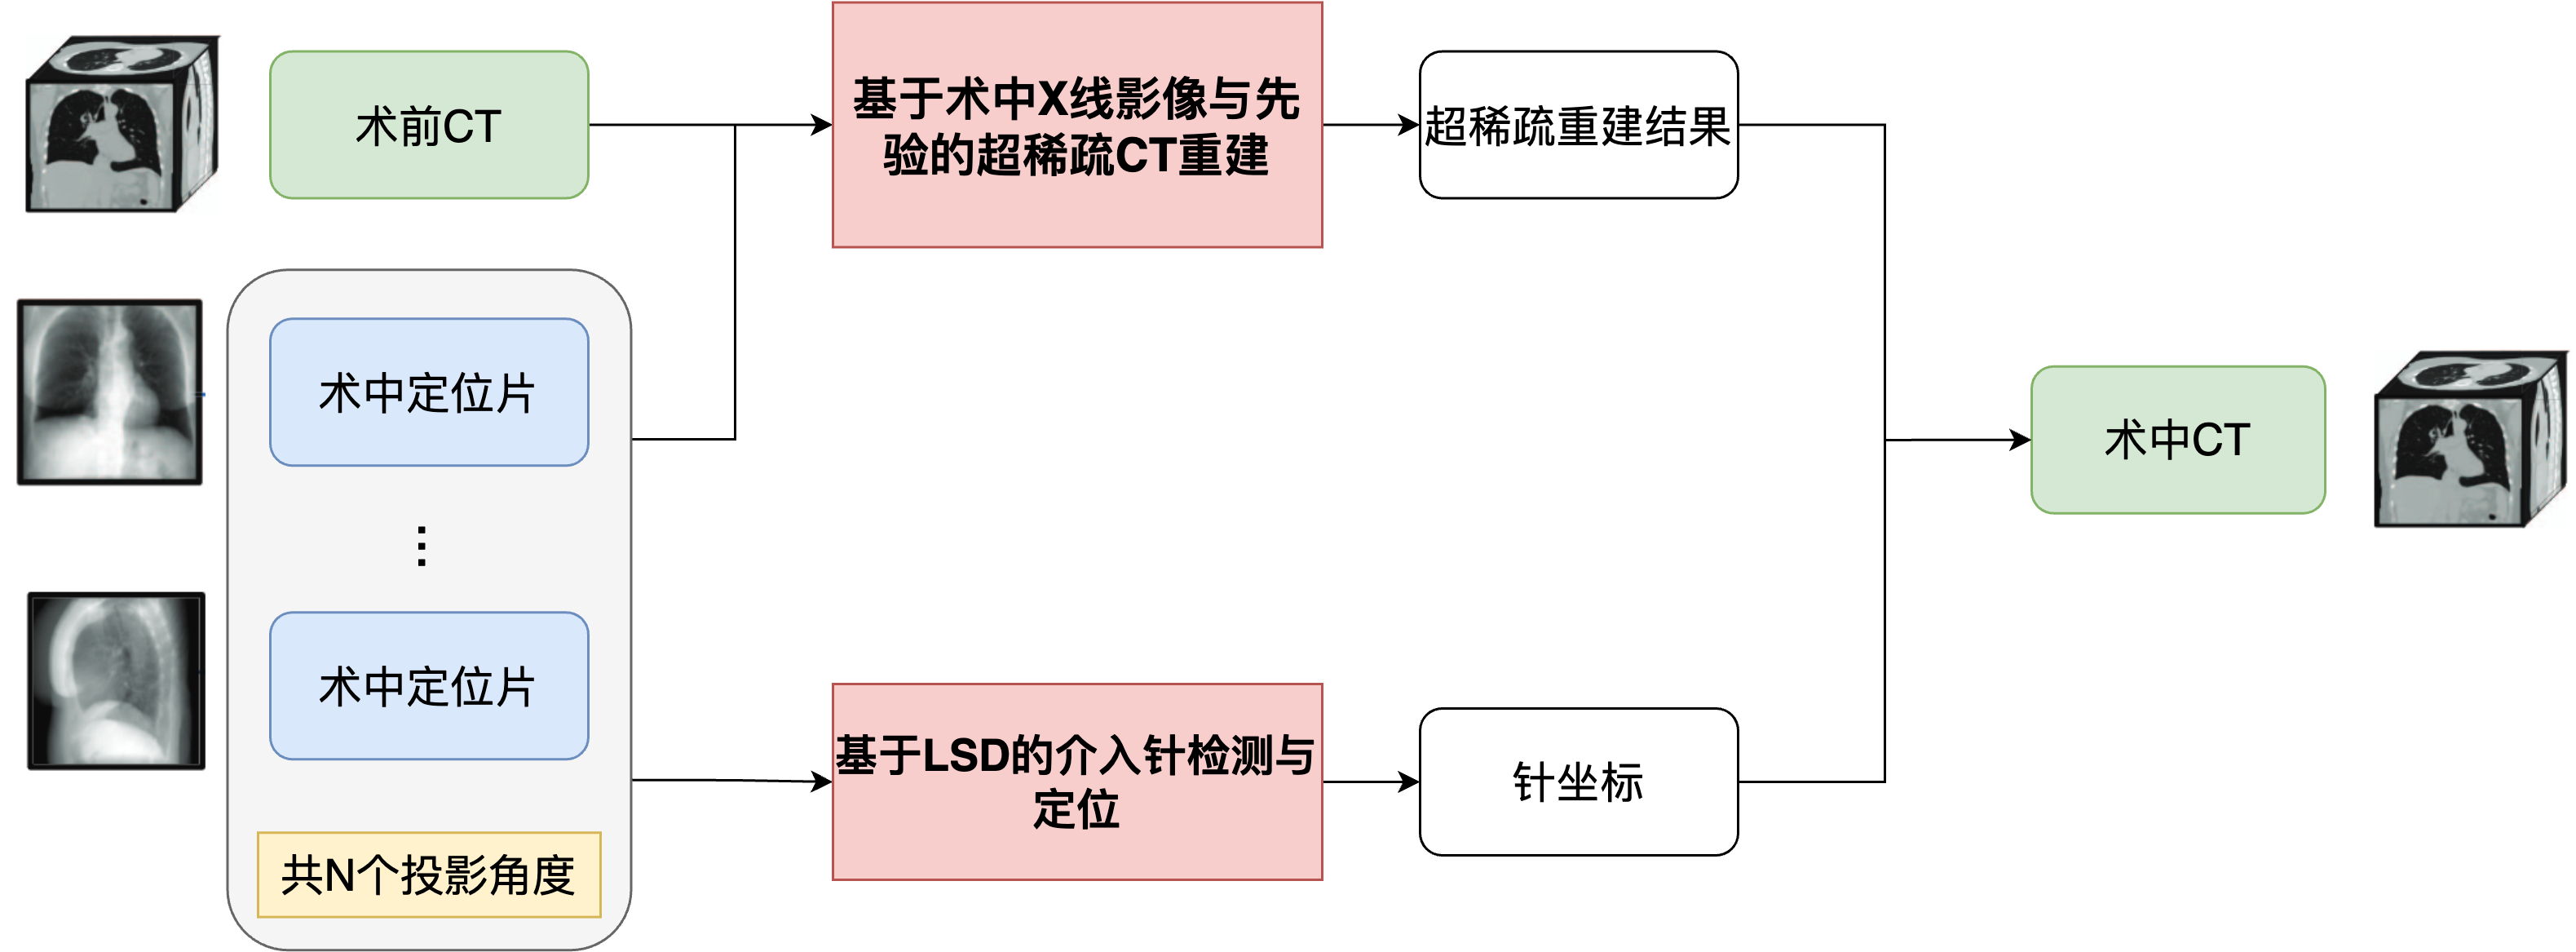
\includegraphics[width=\textwidth]{研究方案.drawio.png}
  \bicaption{本文研究内容示意}{The Overall content of the thesis}
  \label{fig. content}
\end{figure}

\begin{enumerate}
  \item 针对介入手术扫描时间长,医患双方所受辐射剂量大的问题,在术中使用X线定位片代替完整的CT扫描,用于最大化降低扫描剂量。此外,借助术前先验信息,实现了基于Transformer和特征反投影的超稀疏CT重建算法FBFormer(Feature Back-projection Transformer),用于重建术中介入CT影像。该方法通过引入混合的UNet和Transformer架构,提升了术中影像和术前先验图像的特征捕获效果。此外,该方法提出了一种新的特征反投影模块,用于将特征图反投影到原始图像空间,通过引入术中影像的集合信息提升了超稀疏CT重建图像的质量。实验表明,提出的FBFormer模型在介入手术重建任务中取得了最佳的重建效能。
  \item 针对介入针的定位和金属伪影的问题,使用基于LSD的直线检测方法进行图像后处理,该方法通过检测术中定位片影像中的直线结构,在术中三维重建图像中对介入针进行定位,从而避免了CT重建中的金属伪影。实验表明,直线检测方法在介入针的重建图像的精确定位和伪影去除上取得了较好的效果。 %TODO 针检测研究内容
\end{enumerate}
综上所述,本文针对当前介入手术CT引导存在的问题,提出了一种基于深度学习的介入CT重建算法,实现了术中介入CT扫描的实时重建,并在时空分辨率、重建质量和金属伪影抑制等方面取得了较好的效果。本文的研究成果对于提高介入手术的安全性和准确性具有重要的临床应用价值。

\section{本文的组织结构}
本文基于先验信息和术中实时信息相结合的思路,提出了一种基于深度学习的介入CT重建算法,全文共分四章,详细的组织结构如下:

第一章内容为本课题的研究背景和意义。首先概述了CT影像在介入手术中起到的作用和当前介入CT重建算法存在的不足,以引出基于先验信息的实时三维介入CT重建研究的重要价值。之后分别调研了LDCT重建算法的研究现状,包括传统的图像处理方法以及四类不同思路的深度学习算法,并介绍了GAN和Transformer在医学图像处理中的应用。最后简要介绍了直线检测方法的研究现状。最后总结了本文的主要研究内容和贡献。

第二章内容针对当前介入CT重建算法存在的问题,提出了一种基于Transformer和特征反投影模块的深度学习的介入CT重建算法。首先介绍了所提出的基于先验的超稀疏CT重建模型的网络结构,之后介绍了计算机数据模拟的过程和在模拟数据集和临床数据集上的模型效果和泛化性能,最后分析了所构建的重建模型的临床应用价值。

% TODO 第三章内容
第三章内容针对介入手术中的手术器械检测和定位问题,

第四章对本研究所做工作进行了总结,对未来工作进行了展望并提出了未来深入研究的可能方向。

% !TEX root = ../main.tex

\chapter{基于X线影像和先验的超稀疏CT重建}

\section{引言}
自CT被发明以来,降低剂量一直是CT领域的一个重要研究方向。

在此类使用直接深度学习方法进行重建的研究中,有一类比较特殊的问题:超稀疏(Ultra-sparse View)CT重建,或者说使用若干X线定位片生成CT影像的问题。减少投影角度是LDCT的一种实现方式,通常只包含100个投影角度以下的投影角度。而正常剂量的CT,使用FBP算法重建需要几百甚至上千个角度。对于这类稀疏角度CT重建问题,使用MBIR或者深度学习算法更为适合。而其中的极端情况,即仅包含几个投影角度的在深度学习算法出现之前,由于投影图包含的信息过少,几乎没有办法得到有效的结果。得益于神经网络强大的拟合能力,目前也已经有了不少这类问题的研究成果。Shen等人首先提出了PatRecon模型,使用单病人的样本通过二维X线影像生成三维CT断层数据,并且对不同数量扫描角度的X线影像样本做了对比实验,在不同部位的样本上证明了深度学习方法对这一问题的可行性\cite{shenPatientspecificReconstructionVolumetric2019}。Ying等人提出了X2CT模型,该方法利用两个正交的X线影像样本生成CT影像,结合生成对抗损失和投影重建损失函数,取得了比较成熟的效果\cite{yingX2CTGANReconstructingCT2019}。由于在该问题中,输入图像为若干张二维图像,而输出则为三维影像,因此在网络结构的设计上必然存在从二维向三维转换的过程,Ying等人也提出了全新的特征转换方式。Jiang等人使用条件变分自编码器(Conditional Variational Autoencoder,CVAE-GAN),从单个X线影像重建了三维CT影像\cite{jiangReconstruction3DCT2021}。Shen等人提出了几何信息图像重建(Geometry-Informed Image Reconstruction,GIIR),通过将不同投影角度的X线影像特征解耦的方式,实现了一个两步骤的三维CT重建\cite{shenGeometryinformedDeepLearning2022}。

\section{基于Transformer和特征反投影的超稀疏CT重建}
\subsection{FBFormer网络结构}

\subsection{混合的PVT和UNet生成器}

\subsection{特征反投影模块}

\subsection{损失函数}

\section{实验数据与实施细节}

\section{实验结果与分析}

\section{讨论}

\section{本章小结}


% !TEX root = ../main.tex

\chapter{基于LSD的介入针检测与定位}

\section{引言}

\section{基于Transformer和特征饭投影的超稀疏CT重建}


\section{LSD方法}

\section{实验数据与实施细节}

\section{实验结果与分析}

\section{讨论}

\section{本章小结}


% !TEX root = ../main.tex

\chapter{总结与展望}

\section{本文工作总结}

\section{主要贡献}

\section{未来工作展望}


%TC:ignore

% 参考文献
\printbibliography[heading=bibintoc]

% 附录
\appendix

% 附录中图表不加入索引
\captionsetup{list=no}

% 附录内容
% \input{contents/app_maxwell_equations}
% \input{contents/app_flow_chart}

% 结尾部分
\backmatter

% 用于盲审的论文需隐去致谢、发表论文、科研成果、简历

% 致谢
% !TEX root = ../main.tex

\begin{acknowledgements}
  
\end{acknowledgements}


% 发表论文及科研成果
% 盲审论文中,发表论文及科研成果等仅以第几作者注明即可,不要出现作者或他人姓名
% !TEX root = ../main.tex

\begin{achievements}

\subsection*{学术论文}

\begin{bibliolist}{00}
  \item Pei Y, Liu Y, et al. FBFormer: Ultra-sparse CT Reconstruction with Image Prior Using Feature Back-projection and Transformer[J]. IEEE Transactions of Medical Imaging(In Submission).
\end{bibliolist}

\end{achievements}


% % 简历
% \input{contents/resume}

% % 学士学位论文要求在最后有一个大摘要,单独编页码
% \input{contents/digest}

%TC:endignore

\end{document}
